% ch2-laguerre.tex
\documentclass[../main/main]{subfiles}
\small
\begin{document}

\chapter{Laguerre多項式}

\vspace{-180pt}
\begin{figure}[H]
  \begin{flushright}
    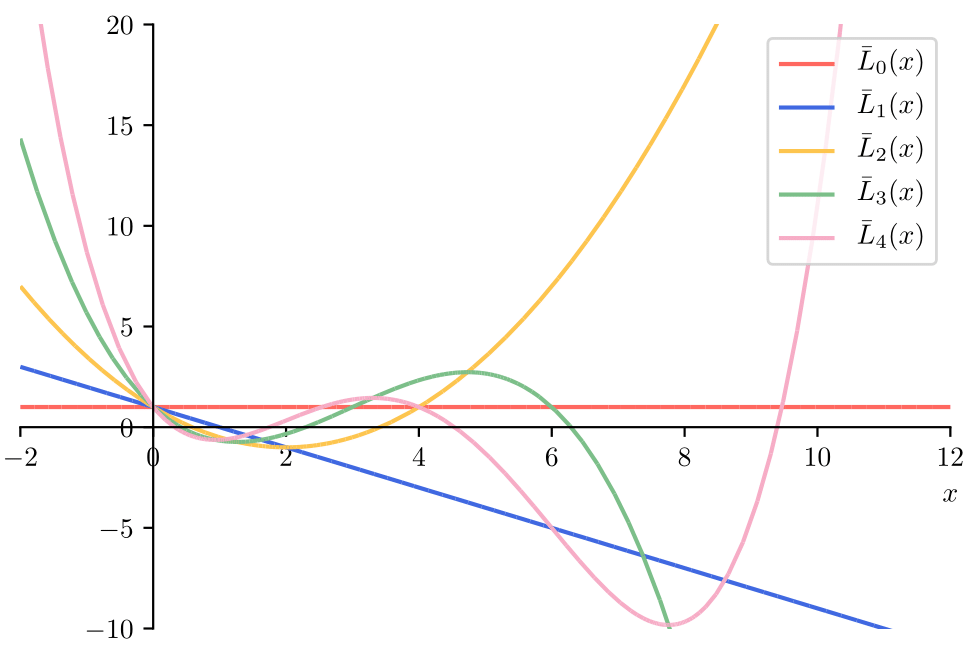
\includegraphics[width=80mm]{../fig/laguerre/laguerre_title.png}
  \end{flushright}
\end{figure}

\vspace{-12pt}
\small
\section{Laguerre多項式}
Laguerre多項式自体は物理への応用に直接用いられることは少なく、
むしろ次節のLaguerre陪多項式の導入のために議論されると考えたほうが良い。

\subsection*{公式集}

\paragraph{母関数}

\begin{equation}\label{eq:Ln-generator}
  g(t, x) = \frac{1}{1-t} \exp \( -\frac{xt}{1-t} \)
	= \sum_{n=0}^\infty \frac{t^n}{n!} L_n (x)
\end{equation}

\paragraph{$x=0$での特殊値}
\begin{equation}
  L_n(0) = n!
\end{equation}

\paragraph{Rodriguesの公式}

\begin{equation}\label{eq:Ln-Rod}
  L_n(x) = e^x \dx{n} (x^n e^{-x})
\end{equation}

\paragraph{一般項}
\begin{equation}\label{eq:Ln-ippan}
  L_n(x) = \sum_{i=0}^n (-1)^i \frac{(n!)^2}{(i!)^2 (n-i)!} x^i
\end{equation}

\paragraph{漸化式}
\begin{equation}\label{eq:Requ}
  L_{n+1} (x) = (2n + 1 - x ) L_n(x) - n^2 L_{n-1}(x)
\end{equation}

\paragraph{微分漸化式}
\begin{equation}\label{eq:Ln-diff-req}
  L_n^\prime (x) - n L_{n-1}^\prime (x) = -n L_{n-1} (x)
\end{equation}

\paragraph{下降演算子}
\begin{equation}\label{eq:Ln-kako}
  \( x \dx{} - n \) L_n(x) = -n^2 L_{n-1} (x)
\end{equation}

\paragraph{上昇演算子}
\begin{equation}\label{eq:Ln-josho}
  \( x \dx{} +n+1-x \) L_n(x) = L_{n+1} (x)
\end{equation}

\paragraph{微分方程式}
\begin{equation}
   x \frac{d^2 L_n(x)}{dx^2} + (1-x) \frac{d L_n(x)}{dx} + n L_n(x) = 0
\end{equation}

\paragraph{自己随伴形}
\begin{equation}
  \dx{} \[ xe^{-x} \dx{} L_n(x) \]  + ne^{-x}L_n(x) = 0
\end{equation}

\paragraph{正規直交性}
\begin{equation}
  \int_0^\infty  e^{-x} L_m(x) L_n(x) \, dx = (n!)^2 \delta_{mn}
\end{equation}


\begin{figure}[bt]
\begin{tabular}{cc}
  \hspace{-5pt}
 \begin{minipage}{0.40\hsize}\small
    \begin{table}[H]
      \centering
      \small
      \caption{\hspace{12pt} Laguerre多項式 $L_n(x)$}
      \begin{tabular}{l}\Hline
        $L_0(x) \ = \ 1$ \\
        $L_1(x) \ = \ -x+1$ \\
        $L_2(x) \ = \ x^2 - 4x + 2$ \\
        $L_3(x) \ = \ -x^3 + 9x^2 - 18x + 6$ \\
        $L_4(x) \ = \ x^4 - 16x^3 + 72x^2 - 96x + 24$ \\
        $L_5(x) \ = \ -x^5 + 25x^4 - 200x^3 + 600x^2 - 600x + 120$ \\\hline
      \end{tabular}
    \end{table}
 \end{minipage}

\hspace{22pt}
 \begin{minipage}{0.60\hsize}
    \begin{figure}[H]
      \centering
      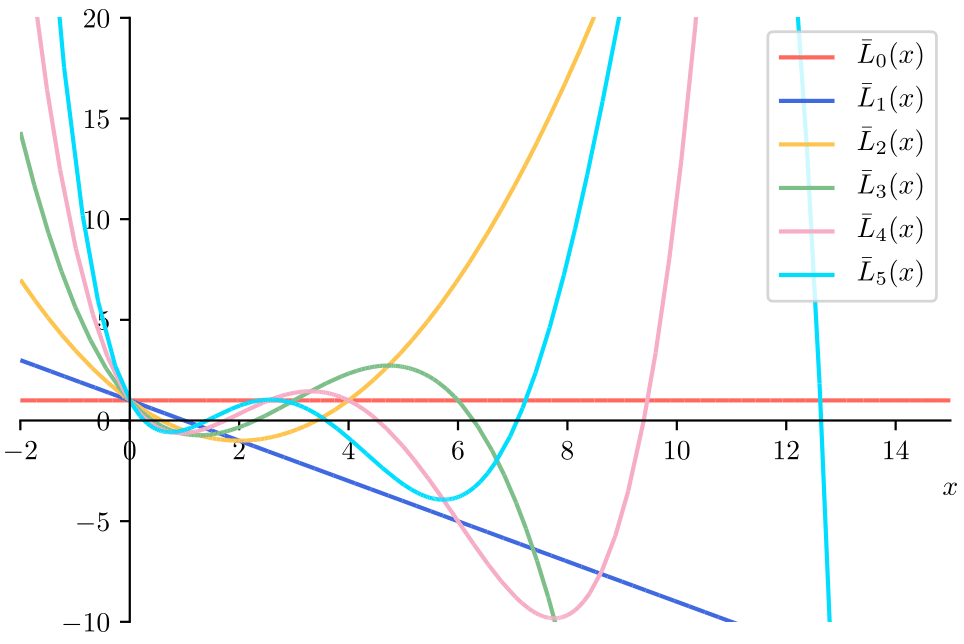
\includegraphics[width=	80mm]{../fig/laguerre/laguerre.png}
      \caption{スケール化されたLaguerre多項式 \ $\bar{L}_n(x) = L_n(x)/n!$}
    \end{figure}
  \end{minipage}
\end{tabular}
\end{figure}


\subsection*{証明}

\paragraph{母関数 $\Longrightarrow$ $x=0$での特殊値}
母関数\eqref{eq:Ln-generator}の両辺に$x=0$を代入すると
\begin{equation}\label{Ln-gen->x=0-En}
  g(t, 0) = \frac{1}{1-t} = \sum_{n=0}^\infty \frac{t^n}{n!} L_n (0)
\end{equation}
ここで\eqref{Ln-gen->x=0-En}の中辺は等比級数の和の公式から$\sum_{n=0}^\infty t^n$であるから、
\eqref{Ln-gen->x=0-En}の右辺と$t^n \ (n\geq 0)$の係数を比較して、次が得られる。
\begin{equation*}
  L_n(0) = n!
\end{equation*}\qed


\paragraph{母関数 $\Longrightarrow$ 一般項}


\small
母関数の式\eqref{eq:Ln-generator}の中辺を$\exp(x) = \sum_{i=0}^\infty \frac{1}{i!} x^i$を用いて展開すると、
\begin{equation*}
  g(t, x) = \sum_{i=0}^\infty \frac{1}{1-t} \frac{1}{i!} \( -\frac{xt}{1-t} \)^i
	= \sum_{i=0}^\infty (-1)^i \frac{x^i}{i!} \frac{t^i}{(1-t)^{i+1}}
\end{equation*}
公式
\footnote{
$f(t) = (1-t)^{-N}$とおくと、$f^\prime (t) = N(1-t)^{-N-1}$, $f^{\prime \prime} (t) = N(N+1) (1-t)^{-N-2}$, $\dots, $ $f^{(m)} (t) = \frac{(N+m-1)!}{(N-1)!} (1-t)^{-N-m}$であるので、
$t=0$の周りでTaylor展開すると
\begin{equation}\label{eq:1F0}
f(t)  = \frac{1}{(1-t)^N}
	= \sum_{m=0}^\infty f^{(m)} (0) \frac{t^m}{m!} 
	=  \sum_{m=0}^\infty \frac{(N+m-1)!}{(N-1)!} \frac{1}{m!} t^m
\end{equation}
なお、
\begin{equation}\label{eq:dx-alpha}
  \dx{\alpha} x^n = \frac{n!}{(n-\alpha)!} x^{n-\alpha}
\end{equation}
}
:
\begin{equation*}
  (1-t)^{-N} = \sum_{m=0}^\infty \frac{(N+m-1)!}{(N-1)!} \frac{t^m}{m!} 
\end{equation*}
から
\begin{align}
  g(t, x) &= \sum_{i=0}^\infty (-1)^i \frac{x^i}{i!} t^i \sum_{m=0}^\infty \frac{(m+i)!}{i!} \frac{t^m}{m!}\notag\\
	&= \sum_{m=0}^\infty \sum_{i=0}^\infty (-1)^i \frac{(m+i)!}{ (i!)^2 \, m!} x^i t^{m+i}
	\label{eq:Ln-gene->ippan}
\end{align}

\vspace{-12pt}
\begin{figure}[H]
  \begin{tabular}{c}
 \begin{minipage}{0.54\hsize}\small
ここで$m+i$を新たに$n$と置き換えて$m, i$についての二重和を$n, i$についての二重和に取りかえる。
$m$について$0$から$\infty$まで、$i$について$0$から$\infty$まで加えていくとき、
二重和は図\ref{fig:laguerre}の黒丸で表した格子点すべてについて実行される。
$n=m+i$であるとき、$n=0, 1, 2, \dots$に対応する全格子点は
図\ref{fig:laguerre}で示した各直線上の点として捉えることができる。
したがって図\ref{fig:laguerre}より、\eqref{eq:Ln-gene->ippan}における二重和は、
$n$について$0$から$\infty$まで、$i$について$0$から$n$までの二重和に
取りかえられることになる。よって、
 \end{minipage}
  
  \begin{minipage}{0.04\hsize}
    \hspace{0pt}
  \end{minipage}

 \begin{minipage}{0.42\hsize}
    \centering
    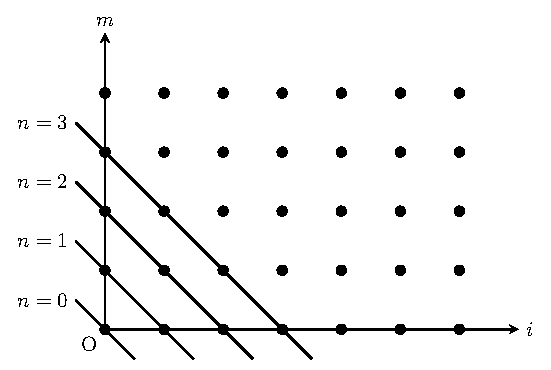
\includegraphics[width=60mm]{../TikZ/laguerre/laguerre.pdf}
    \caption{二重和の取りかえ方}
    \label{fig:laguerre}
 \end{minipage}
  \end{tabular}
\end{figure}

\vspace{-12pt}
\begin{equation*}
  g(t, x) = \sum_{n=0}^\infty \sum_{i=0}^n (-1)^i \frac{n!}{(i!)^2(n-i)!} x^i t^{n}
	= \sum_{n=0}^\infty \sum_{i=0}^n \frac{t^n}{n!} (-1)^i \frac{(n!)^2}{(i!)^2(n-i)!} x^i t^{n} \notag\\
\end{equation*}
母関数の右辺\eqref{eq:Ln-generator}と比較して
\begin{equation*}
  L_n(x) = \sum_{i=0}^n (-1)^i \frac{(n!)^2}{(i!)^2 (n-i)!} x^i
\end{equation*}\qed


\paragraph{Rodriguesの公式 $\Longrightarrow$ 母関数}
Cauchyの積分公式\eqref{eq:cauchy-diff}を用いてRodriguesの公式\eqref{eq:Ln-Rod}を積分形式に書き換えると、
\begin{equation*}
  L_n(x) = e^x \frac{n!}{2\pi i} \int_C \frac{\xi^n e^{-\xi}}{(\xi-x)^{n+1}}d \xi
\end{equation*}
積分経路$C$は$\xi=x$の周りを正の方向に回るようにとる。よって、
\begin{align*}
  \sum_{n=0}^\infty \frac{t^n}{n!} L_n (x)
	&= \sum_{n=0}^\infty \frac{t^n}{n!} \cdot
		e^x \frac{n!}{2\pi i} \int_C \frac{\xi^n e^{-\xi}}{(\xi-x)^{n+1}}d \xi \notag\\
	&= e^x  \frac{1}{2\pi i} \int_C \frac{e^{-\xi}}{\xi-x} 
		\sum_{n=0}^\infty \( \frac{\xi t}{\xi -x} \)^n d\xi \notag
\end{align*}
級数が収束するために$|t|$が十分小さいものとすると、等比級数の和の公式から
\begin{align*}
  \sum_{n=0}^\infty \frac{t^n}{n!} L_n (x)
	&= e^x  \frac{1}{2\pi i} \int_C \frac{e^{-\xi}}{\xi-x} \cdot
		\frac{1}{1-\frac{\xi t}{\xi - x}} d\xi \notag\\
	&= \frac{e^x}{1-t} \cdot \frac{1}{2\pi i} \int_C \frac{e^{-\xi}}{ \xi - \frac{x}{1-t} } d\xi
\end{align*}
被積分関数の極$\xi=\frac{x}{1-t}$が、$t$が十分小さく、$C$の内部にあるとすると、留数定理より
\begin{equation*}
  \sum_{n=0}^\infty \frac{t^n}{n!} L_n (x)
	= \frac{e^x}{1-t} \cdot \frac{1}{2\pi i} \cdot 2 \pi i \[ e^{-\xi} \]_{\xi = \frac{x}{1-t}}
	= \frac{1}{1-t} \exp \( - \frac{xt}{1-t} \)
\end{equation*}\qed



\paragraph{Rodriguesの公式 $\Longrightarrow$ 一般項}

Rodriguesの公式\eqref{eq:Ln-Rod}をLeibnizの公式
\footnote{
\textbf{Leibnizの公式}
\begin{equation}\label{eq:Leibniz}
\dx{n} (f(x) g(x)) = \sum_{i=0}^{n} \binom{n}{i} f^{(n-i)} (x) g^{(i)} (x)
\end{equation}
}
で展開する。
\begin{align*}
  L_n(x) &= e^x \sum_{i=0}^n \binom{n}{i} \( \dx{n-i} x^n \)  \( \dx{i} e^{-x}\) \\
	&= e^x \sum_{i=0}^n \frac{n!}{i! (n-i)!} \cdot \frac{n!}{i!} x^i \cdot (-1)^i e^{-x}  
		\qquad (\eqref{eq:dx-alpha}を用いた)\quad\\
	&= \sum_{i=0}^n (-1)^i \frac{(n!)^2}{(i!)^2 (n-i)!} x^i 
\end{align*}\qed

\paragraph{母関数 $\Longrightarrow$ 漸化式}

母関数\eqref{eq:Ln-generator}の左, 右辺を$t$で偏微分して
\begin{equation}\label{eq:Ln-6g}
  \frac{\6 g(t, x)}{\6 t} = \sum_{n=1}^\infty \frac{t^{n-1}}{(n-1)!} L_n (x)
	=  \sum_{n=0}^\infty \frac{t^n}{n!} L_{n+1} (x)
\end{equation}
一方、母関数\eqref{eq:Ln-generator}の左, 中辺の対数をとると、
\begin{equation*}
  \log g(t, x) + \log (1-t) + \frac{xt}{1-t} = 0
\end{equation*}
両辺を$t$で偏微分すると、
\begin{gather*}
  \frac{1}{g(t, x)} \frac{\6 g(t, x)}{\6 t} - \frac{1}{1-t} + \frac{x}{(1-t)^2} = 0  \\
  \therefore (1-t)^2 \frac{\6 g(t, x)}{\6 t} + (x-1+t) g(t, x) = 0
\end{gather*}
これに母関数の式\eqref{eq:Ln-generator}の右辺および\eqref{eq:Ln-6g}を代入すると、
\begin{gather*}
  (1-t)^2 \sum_{n=0}^\infty \frac{t^n}{n!} L_{n+1} (x)
	+(x-1+t) \sum_{n=0}^\infty \frac{t^n}{n!} L_n (x) = 0\\
  \sum_{n=0}^\infty \frac{t^n}{n!} L_{n+1} (x) 
	- 2 \sum_{n=0}^\infty \frac{t^{n+1}}{n!} L_{n+1} (x)
	+ \sum_{n=0}^\infty \frac{t^{n+2}}{n!} L_{n+1} (x)
	  +(x-1) \sum_{n=0}^\infty \frac{t^n}{n!} L_n (x)
	  + \sum_{n=0}^\infty \frac{t^{n+1}}{n!} L_n (x)  = 0
\end{gather*}
ここで$\frac{1}{(負の整数)!}=0$と約束して$t$の指数をそろえると
\begin{gather*}
  \sum_{n=0}^\infty \frac{t^n}{n!} L_{n+1} (x) 
	- 2 \sum_{n=0}^\infty \frac{t^{n}}{(n-1)!} L_{n} (x)
	+ \sum_{n=0}^\infty \frac{t^{n}}{(n-2)!} L_{n-1} (x)
	  +(x-1) \sum_{n=0}^\infty \frac{t^n}{n!} L_n (x)
	  + \sum_{n=0}^\infty \frac{t^{n}}{(n-1)!} L_{n-1} (x)  = 0\\ \therefore
  \sum_{n=0}^\infty \frac{t^n}{n!} 
	\[  L_{n+1} (x) - (2n + 1 - x ) L_n(x) + n^2 L_{n-1}(x) \] = 0
\end{gather*}
$t^n \ (n \geq 0)$の係数を比較することで次を得る:
\begin{equation*}
   L_{n+1} (x) = (2n + 1 - x ) L_n(x) - n^2 L_{n-1}(x)
\end{equation*}\qed

\paragraph{母関数 $\Longrightarrow$ 微分漸化式}

母関数の式\eqref{eq:Ln-generator}の両辺を$x$で偏微分すると
\begin{equation*}
  \frac{\6 g(t, x)}{\6 x} 
	= -\frac{t}{1-t} g(t, x) = \sum_{n=0}^\infty \frac{t^n}{n!} L_n^\prime (x)
\end{equation*}
$g(t, x)$に母関数の式\eqref{eq:Ln-generator}の右辺を代入すると、
\begin{gather*}
  -\frac{t}{1-t} \sum_{n=0}^\infty \frac{t^n}{n!} L_n (x)
	= \sum_{n=0}^\infty \frac{t^n}{n!} L_n^\prime (x)\\ \therefore
  - \sum_{n=0}^\infty \frac{t^{n+1}}{n!} L_n (x)
	= \sum_{n=0}^\infty \frac{t^n}{n!} L_n^\prime (x)
	  - \sum_{n=0}^\infty \frac{t^{n+1}}{n!} L_n^\prime (x)
\end{gather*}
$\frac{1}{(負の整数)!}=0$と約束して$t$の指数をそろえると
\begin{gather*}
  - \sum_{n=0}^\infty \frac{t^{n}}{(n-1)!} L_{n-1} (x)
	= \sum_{n=0}^\infty \frac{t^n}{n!} L_n^\prime (x)
	  - \sum_{n=0}^\infty \frac{t^n}{(n-1)!} L_{n-1}^\prime (x) \\ \therefore
  \sum_{n=0}^\infty \frac{t^n}{n!} 
	\[ L_n^\prime (x) - n L_{n-1}^\prime (x) + n L_{n-1} (x)  \] = 0
\end{gather*}
$t^n \ (n \geq 0)$の係数を比較することで次を得る。
\begin{equation*}
  L_n^\prime (x) - n L_{n-1}^\prime (x) = - n L_{n-1} (x)
\end{equation*}\qed

\paragraph{漸化式, 微分漸化式 $\Longrightarrow$ 下降演算子}
下降演算子の式は、漸化式\eqref{eq:Requ}と微分漸化式\eqref{eq:Ln-diff-req}を組み合わせることで
示すことができる。
まず漸化式\eqref{eq:Requ}の両辺を$x$で微分した
\begin{equation*}
  L_{n+1}^\prime (x) = -L_n(x) + (2n + 1 - x ) L_n^\prime (x) - n^2 L_{n-1}^\prime (x)
\end{equation*}
と\eqref{eq:Ln-diff-req}から$L_{n-1}^\prime (x)$を消去すると、
\begin{equation}\label{eq:Ln-zen->kako-1}
  L_{n+1}^\prime (x) - (n+1-x) L_n^\prime (x) + L_n(x) + n^2 L_{n-1}(x) = 0
\end{equation}
次に微分漸化式\eqref{eq:Ln-diff-req}で$n \to n+1$と書き換えると
\begin{equation}\label{eq:Ln-zen->kako-2}
  L_{n+1}^\prime (x) - (n+1) L_{n}^\prime (x) = - (n+1)L_{n} (x)
\end{equation}
得られた\eqref{eq:Ln-zen->kako-1}, \eqref{eq:Ln-zen->kako-2}式から
$L_{n+1}^\prime (x)$を消去すると
\begin{gather*}
  x L_n^\prime (x) - n L_{n} (x) = -n^2 L_{n-1}(x) \qquad \therefore
	\( x \dx{} - n \) L_n(x) = -n^2 L_{n-1} (x)
\end{gather*}\qed


\paragraph{漸化式, 下降演算子 $\Longrightarrow$ 上昇演算子}

漸化式\eqref{eq:Requ}と下降演算子\eqref{eq:Ln-kako}から
$-n^2 L_{n-1}(x)$を消去することで直ちに
\begin{equation*}
  \( x \dx{} +n+1-x \) L_n(x) = L_{n+1} (x)
\end{equation*}\qed

\paragraph{昇降演算子 $\Longrightarrow$ 微分方程式}

下降演算子の式\eqref{eq:Ln-kako}で$n \to n+1$とした式
\begin{equation}\label{eq:Ln-shoko->bibun}
  \[ x \dx{} - (n+1) \] L_{n+1}(x) = -(n+1)^2 L_{n} (x)
\end{equation}
を用いるために、上昇演算子の式\eqref{eq:Ln-josho}の両辺に
$\[ x \dx{} - (n+1) \]$を左から作用させると、
\begin{equation*}
  \[ x \dx{} - (n+1) \] \( x \dx{} +n+1-x \) L_n(x) = \( x \dx{} - (n+1) \) L_{n+1} (x)
\end{equation*}
演算子$f$について$\(\dx{}\) f = \frac{df}{dx} + f \dx{} $であることなどに注意して左辺を展開し、
右辺に\eqref{eq:Ln-shoko->bibun}を代入して整理すると
\begin{gather*}
  \[ x^2 \dx{2} + x(1-x) \dx{} + nx \] L_n(x) = 0 \qquad \therefore
  x \frac{d^2 L_n(x)}{dx^2} + (1-x) \frac{d L_n(x)}{dx} + n L_n(x) = 0
\end{gather*}
また、この方程式は次のようにも変形できる。
\begin{equation*}
  \dx{} \[ xe^{-x} \dx{} L_n(x) \]  + ne^{-x}L_n(x) = 0
\end{equation*}\qed


\paragraph{母関数 $\Longrightarrow$ 直交性}

母関数\eqref{eq:Ln-generator}の右辺から
\begin{align}
  \int_0^\infty e^{-x}  g(s, x)g(t, x) dx
	&= \int_0^\infty e^{-x} \( \sum_{m=0}^\infty \frac{s^m}{m!} L_m (x) \)
		\( \sum_{n=0}^\infty \frac{t^n}{n!} L_n (x) \)  dx\notag\\
	&= \sum_{m=0}^\infty \sum_{n=0}^\infty \frac{s^m t^n}{m! n!} \int_0^\infty e^{-x} L_m (x) L_n (x) \, dx
	\label{eq:Ln-gene->seiki-1}
\end{align}
一方、母関数\eqref{eq:Ln-generator}の中辺から
\begin{align}
   \int_0^\infty e^{-x}  g(s, x)g(t, x) dx
	&= \int_0^\infty e^{-x} \frac{1}{1-s} \exp \( -\frac{xs}{1-s} \)
	 \frac{1}{1-t} \exp \( -\frac{xt}{1-t} \) dx \notag\\
	&= \frac{1}{(1-s)(1-t)} \int_0^\infty \exp \left\{ - \frac{1-st}{(1-s)(1-t)}x \right\} dx \notag\\
	&= -\frac{1}{1-st} \[ \exp \left\{ - \frac{1-st}{(1-s)(1-t)}x \right\} \]_0^\infty \notag\\
	&= \frac{1}{1-st} \notag\\
	&= \sum_{n=0}^\infty s^n t^n \qquad (等比級数の和の公式より) \notag\\
	&= \sum_{m=0}^\infty \sum_{n=0}^\infty \frac{s^m t^n}{m! n!} (n!)^2 \, \delta_{mn}
	\label{eq:Ln-gene->seiki-2}
\end{align}
\eqref{eq:Ln-gene->seiki-1}, \eqref{eq:Ln-gene->seiki-2}を比較することで次を得る。
\begin{equation*}
  \int_0^\infty e^{-x} L_m(x) L_n(x)  \, dx = (n!)^2 \, \delta_{mn}
\end{equation*}

%%%%%%%%%%%%%%%%%%%%%%%%%%%%%%%%%%%%%%%%%%%%%%%%%%%%%%%%

\section{Laguerre陪多項式}

Laguerre陪多項式は水素原子のSchr\"{o}dinger方程式を球座標$(r, \theta, \varphi)$で解く際に、
解の$r$依存性として現れる多項式である( 問題[3-1]] )。
Laguerre陪多項式$L_n^k(x)$の定義は実に多くの流儀がある。
さらに当然であるが流儀によってそれが満たす公式の形も変わってしまう。
これでは議論の術がなくなってしまうので、本稿では
Laguerre多項式$L_n(x)$の$k$階導関数としてLaguerre陪多項式$L_n^k(x)$を定義することにする
\footnote{J.J.Sakurai『現代の量子力学(上, 下)』などの量子力学の教科書や
多くの量子化学の教科書ではこの流儀が採用されている。}。
どれかひとつの流儀を理解しておけば、
他の流儀における公式は容易に類推することができる。
なお、Laguerre陪多項式についての公式で$k=0$とすると
Laguerre多項式についての公式と一致することを強調しておく。

\subsection*{公式集}
\paragraph{定義}
\begin{equation}\label{eq:Lnk-def}
  L_n^k(x) \equiv \dx{k} L_n(x)
\end{equation}

\paragraph{Rodriguesの公式}
\begin{equation}\label{eq:Lnk-Rod}
  L_n^k(x) = \dx{k} e^x \dx{n} (x^n e^{-x})
\end{equation}

\paragraph{Rodriguesの公式II}
\begin{equation}\label{eq:Lnk-RodII}
  L_n^k(x) = (-1)^k \frac{n!}{(n-k)!} e^x x^{-k} \dx{n-k} ( x^n e^{-x} )
\end{equation}

\paragraph{一般項}
\begin{equation}\label{eq:Lnk-ippan}
  L_n^k(x) = \sum_{i=0}^{n-k} (-1)^{k+i} \frac{(n!)^2}{i! (i+k)! (n-k-i)!} x^i
\end{equation}

\paragraph{母関数}
\begin{equation}\label{eq:Lnk-gene}
  g(t, x) 
	= \frac{(-1)^k}{(1-t)^{k+1}} \exp\( -\frac{xt}{1-t} \)
	= \sum_{n=k}^\infty \frac{t^{n-k}}{n!} L_n^k(x)
\end{equation}

\paragraph{$x=0$における特殊値}
\begin{equation}\label{eq:Lnk-x=0}
  L_n^k(0) = (-1)^k \frac{(n!)^2}{(n-k)! k!}
\end{equation}

\paragraph{漸化式}
\begin{equation}\label{eq:Lnk-req}
  \( 1-\frac{k}{n+1} \) L_{n+1}^k (x) + (x+k-2n-1) L_n^k(x) + n^2 L_{n-1}^k (x) = 0
\end{equation}

\paragraph{微分漸化式}
\begin{equation}\label{eq:Lnk-diff-req}
  \frac{d L_n^k (x)}{dx} = n \[ \frac{d L_{n-1}^k (x)}{dx} - L_{n-1}^k (x) \]
\end{equation}

\paragraph{下降演算子}
\begin{equation}\label{eq:Lnk-kako}
  \( x \dx{} -n +k \) L_n^k(x) = -n^2 L_{n-1}^k (x)
\end{equation}

\paragraph{上昇演算子}
\begin{equation}\label{eq:Lnk-josho}
  \( x\dx{} -x +n+1 \) L_n^k(x) = \( 1-\frac{k}{n+1} \) L_{n+1}^k (x)
\end{equation}

\paragraph{微分方程式}
\begin{equation}
  x \frac{d^2 L_n^k(x)}{dx^2} + (k+1-x) \frac{d L_n^k(x)}{dx} + (n-k) L_n^k(x) = 0
\end{equation}

\paragraph{自己随伴形}
\begin{equation}
  \dx{} \( x^{k+1} e^{-x} \frac{d L_n^k(x)}{dx} \) + (n-k) x^k e^{-x} L_n^k(x) = 0
\end{equation}


\paragraph{直交性}
\begin{equation}\label{Lnk-chokko}
  \int_0^\infty x^k e^{-x} L_m^k(x) L_n^k(x) dx = \frac{(n!)^3}{(n-k)!} \delta_{mn}
\end{equation}

\begin{table}[t]
      \centering
      \caption{Laguerre陪多項式 $L_n^k(x)$}\small
      \begin{tabular}{l}\Hline
        $L_1^1(x) \ = \ -1$ \\\hdashline
        $L_2^1(x) \ = \ 2x-2$ \\
        $L_2^2(x) \ = \ 2$ \\\hdashline
        $L_3^1(x) \ = \ -3x^2 + 18x - 18$ \\
        $L_3^2(x) \ = \ -6x + 18$ \\
        $L_3^3(x) \ = \ -6$ \\\hdashline
        $L_4^1(x) \ = \ 4x^3 - 48x^2 + 144x - 96$ \\
        $L_4^2(x) \ = \ 12x^2 - 96x + 144$ \\
        $L_4^3(x) \ = \ 24x-96$\\
        $L_4^4(x) \ = \ 24$\\\hline
      \end{tabular}
\end{table}

\subsection*{証明}

\paragraph{Rodriguesの公式 $\Longrightarrow$ 一般項}

Rodriguesの公式\eqref{eq:Lnk-Rod}は$L_n^k(x)$の定義\eqref{eq:Lnk-def}に
そのまま$L_n(x)$のRodriguesの公式\eqref{eq:Ln-Rod}を代入したものである。
したがって、定義\eqref{eq:Lnk-def}にしたがい、
$L_n(x)$の一般項\eqref{eq:Ln-ippan}の$k$階導関数が
\eqref{eq:Lnk-ippan}になることを確認すればよい。
\begin{alignat*}{2}
  L_n^k(x) &= \dx{k} L_n(x) 
		\overset{\eqref{eq:Ln-ippan}}{=} \dx{k} \sum_{i=0}^n (-1)^i \frac{(n!)^2}{(i!)^2 (n-i)!} x^i \\
	&= \sum_{i=k}^n (-1)^i \frac{(n!)^2}{(i!)^2 (n-i)!}\cdot \frac{i!}{(i-k)!} x^{i-k}
		&\quad& (\eqref{eq:dx-alpha} を用いた)\\
	&= \sum_{i=0}^{n-k} (-1)^{k+i} \frac{(n!)^2}{i! (i+k)! (n-k-i)!} x^i
		&& (i \to k+i と変換した)
\end{alignat*}\qed

\paragraph{Rodriguesの公式II $\Longrightarrow$ 一般項}
\hspace{-6pt}\footnote{Rodriguesの公式とRodriguesの公式IIが等価であることは、
両者から導かれる一般項が一致することより認めることにする。}\hspace{6pt}
Rodriguesの公式II \eqref{eq:Lnk-RodII}をLeibnizの公式\eqref{eq:Leibniz}により展開する。
\begin{align*}
  L_n^k(x) 
	&=  (-1)^k \frac{n!}{(n-k)!} e^x x^{-k} \sum_{i=0}^{n-k} 
		\binom{n-k}{i} \( \dx{n-k-i} \, x^n \) \( \dx{i}  e^{-x} \) \\
	&= (-1)^k \frac{n!}{(n-k)!} e^x x^{-k} \sum_{i=0}^{n-k} 
		\frac{(n-k)!}{i! (n-k-i)!} \cdot \frac{n!}{(i+k)!} x^{i+k} \cdot (-1)^i e^{-x} 
		\qquad (\eqref{eq:dx-alpha} を用いた)\\
	&= \sum_{i=0}^{n-k} (-1)^{k+i} \frac{(n!)^2}{i! (i+k)! (n-k-i)!} x^i
\end{align*}\qed


\paragraph{Rodriguesの公式II $\Longrightarrow$ 母関数}

Rodriguesの公式II\eqref{eq:Lnk-RodII}から、
\begin{align*}
  \sum_{n=k}^\infty \frac{t^{n-k}}{n!} L_n^k(x)
	&= \sum_{n=k}^\infty \frac{t^{n-k}}{n!}\cdot  (-1)^k \frac{n!}{(n-k)!} e^x x^{-k} 
		\dx{n-k} ( x^n e^{-x} ) \notag\\
	&= (-1) ^k e^x x^{-k} \sum_{n=k}^\infty \frac{t^{n-k}}{(n-k)!}  \dx{n-k} ( x^n e^{-x} ) \notag\\
	&= (-1)^k e^x x^{-k} \sum_{n=0}^\infty \frac{t^n}{n!} \dx{n} ( x^{n+k} e^{-x} ) \notag
\end{align*}
経路$C$を、点$\xi = x$の周りを正の向きに回るものとすると、
		Cauchyの積分公式\eqref{eq:cauchy-diff}より
\begin{align*}
  \sum_{n=k}^\infty \frac{t^{n-k}}{n!} L_n^k(x)
	&= (-1)^k e^x x^{-k} \sum_{n=0}^\infty \frac{t^n}{n!} \cdot
		\frac{n!}{2\pi i} \int_C \frac{\xi^{n+k} e^{-\xi} }{(\xi - x)^{n+1}} d\xi \notag\\
	&= (-1)^k e^x x^{-k} \frac{1}{2\pi i} \int_C
		\frac{\xi^k e^{-\xi}}{\xi -x} \sum_{n=0}^\infty \( \frac{\xi t}{\xi - x} \)^n d\xi
\end{align*}
級数が収束するために$|t|$が十分小さいものとすると、等比級数の和の公式から
\begin{align*}
  \sum_{n=k}^\infty \frac{t^{n-k}}{n!} L_n^k(x)
	&= (-1)^k e^x x^{-k} \frac{1}{2\pi i} \int_C
		\frac{\xi^k e^{-\xi}}{\xi -x} \cdot \frac{1}{1- \frac{\xi t}{\xi - x} } d\xi \notag\\
	&= (-1)^k e^x x^{-k} \frac{1}{1-t} \cdot \frac{1}{2\pi i} \int_C
		\frac{\xi^k e^{-\xi}}{\xi - \frac{x}{1-t}}  d\xi
\end{align*}
被積分関数の極$\xi=\frac{x}{1-t}$が、$t$が十分小さく、$C$の内部にあるとすると、留数定理より
\begin{align*}
  \sum_{n=k}^\infty \frac{t^{n-k}}{n!} L_n^k(x)
	&= (-1)^k e^x x^{-k} \frac{1}{1-t} \cdot \frac{1}{2\pi i} 
		\cdot 2\pi i \[ \xi^k e^{-\xi} \]_{\xi = \frac{x}{1-t}} \notag\\
	&= \frac{(-1)^k}{(1-t)^{k+1}} \exp \( -\frac{xt}{1-t} \)
\end{align*}\qed

\paragraph{母関数 $\Longrightarrow$ $x=0$における特殊値}

母関数\eqref{eq:Lnk-gene}において$x=0$を代入すると、
\begin{equation}\label{eq:Lnk-gene->x=0}
   g(t, 0) 
	= \frac{(-1)^k}{(1-t)^{k+1}} 
	= \sum_{n=k}^\infty \frac{t^{n-k}}{n!} L_n^k(0)
\end{equation}
ここで、\eqref{eq:Lnk-gene->x=0}の中辺は\eqref{eq:1F0}を用いて
\begin{equation*}
  \frac{(-1)^k}{(1-t)^{k+1}}  
	= (-1)^k \sum_{n=0}^\infty \frac{(n+k)!}{n! k!} t^n
	= (-1)^k \sum_{n=k}^\infty \frac{n!}{(n-k)! k!} t^{n-k}
	= \sum_{n=k}^\infty \frac{t^{n-k}}{n!} \cdot (-1)^k \frac{(n!)^2}{(n-k)! k!}
\end{equation*}
となる。したがって、\eqref{eq:Lnk-gene->x=0}の右辺と比較して次を得る。
\begin{equation*}
  L_n^k(0) = (-1)^k \frac{(n!)^2}{(n-k)! k!}
\end{equation*}

\paragraph{母関数 $\Longrightarrow$ 漸化式}

母関数\eqref{eq:Lnk-gene}の左, 右辺を$t$で偏微分して
\begin{equation}\label{eq:Lnk-gene->req-6t}
  \frac{\6 g(t, x)}{\6 t} 
	= \sum_{n=k+1}^\infty \frac{n-k}{n!}  t^{n-k-1} L_n^k(x)
	= \sum_{n=k}^\infty \frac{n-k+1}{(n+1)!} t^{n-k} L_{n+1}^k(x)
\end{equation}
一方、母関数\eqref{eq:Lnk-gene}の左, 中辺の対数をとると、
\begin{equation*}
  \log g(t, x) = - (k+1) \log (1-t) + k \log (-1) - \frac{xt}{1-t}
\end{equation*}
となる
\footnote{ここで対数の真数が負になっている項$\log (-1)$が現れているが、これは計算を楽にするために
形式的に書いていると考えればよい。
それが疑問であれば、複素関数として$\log (-1) = (2n+1)\pi i \ (n \in \mathbb{Z})$と解釈すればよい。
いずれにせよ後に$t$で偏微分する時に消えるので憂う必要はない。}
。
両辺を$t$で偏微分すると、
\begin{gather*}
  \frac{1}{g(t, x)} \frac{\6 g(t, x)}{\6 t} = \frac{k+1}{1-t} - \frac{x}{(1-t)^2} \\\notag \therefore
  (1-t)^2 \frac{\6 g(t, x)}{\6 t} = \{ (k+1-x) - (k+1)t \} g(t, x)
\end{gather*}
これに母関数\eqref{eq:Lnk-gene}の右辺および\eqref{eq:Lnk-gene->req-6t}を代入すると、
\begin{equation*}
  (1-t)^2 \sum_{n=k}^\infty \frac{n-k+1}{(n+1)!} t^{n-k} L_{n+1}^k(x)
	= \{ (k+1-x) - (k+1)t \} \sum_{n=k}^\infty \frac{t^{n-k}}{n!} L_n^k(x) 
\end{equation*}
\begin{gather*} \therefore
  \sum_{n=k}^\infty \frac{n-k+1}{(n+1)!} t^{n-k} L_{n+1}^k(x)
		-2 \sum_{n=k}^\infty \frac{n-k+1}{(n+1)!} t^{n-k+1} L_{n+1}^k(x)
		+ \sum_{n=k}^\infty \frac{n-k+1}{(n+1)!} t^{n-k+2} L_{n+1}^k(x) \notag\\\hspace{60pt}
	= (k+1-x) \sum_{n=k}^\infty \frac{t^{n-k}}{n!} L_n^k(x) 
		-(k+1) \sum_{n=k}^\infty \frac{t^{n-k+1}}{n!} L_n^k(x) 
\end{gather*}
$L_{k-1}^k (x) = 0$を用いて$t$の指数をそろえると
\begin{gather*}
  \sum_{n=k}^\infty \frac{n-k+1}{(n+1)!} t^{n-k} L_{n+1}^k(x)
		-2 \sum_{n=k}^\infty \frac{n-k}{n!} t^{n-k} L_{n}^k(x)
		+ \sum_{n=k}^\infty \frac{n-k-1}{(n-1)!} t^{n-k} L_{n-1}^k(x) \notag\\\hspace{60pt}
	= (k+1-x) \sum_{n=k}^\infty \frac{t^{n-k}}{n!} L_n^k(x) 
		-(k+1) \sum_{n=k}^\infty \frac{t^{n-k}}{(n-1)!} L_{n-1}^k(x) 
\end{gather*}
\begin{gather*} \therefore
  \sum_{n=k}^\infty \frac{t^{n-k}}{(n+1)!} \[ (n+1-k) L_{n+1}^k(x) 
		+ (n+1) (x+k-2n-1) L_n^k(x)  + (n+1)n \cdot n L_{n-1}^k(x) \] = 0 
\end{gather*}
$t^{n-k} \ (n \geq k)$の係数を比較することで次を得る:
\begin{equation*}
  \( 1-\frac{k}{n+1} \) L_{n+1}^k (x) + (x+k-2n-1) L_n^k(x) + n^2 L_{n-1}^k (x) = 0
\end{equation*}\qed

\paragraph{母関数 $\Longrightarrow$ 微分漸化式}


母関数\eqref{eq:Lnk-gene}の両辺を$x$で偏微分すると
\begin{equation*}
  \frac{\6 g(t, x)}{\6 x}
	= -\frac{t}{1-t} g(t, x)
	= \sum_{n=k}^\infty \frac{t^{n-k}}{n!} \frac{d L_n^k (x)}{dx}
\end{equation*}
$g(t, x)$に母関数\eqref{eq:Lnk-gene}の右辺を代入すると、
\begin{gather*}
  -\frac{t}{1-t} \sum_{n=k}^\infty \frac{t^{n-k}}{n!} L_n^k(x)
	= \sum_{n=k}^\infty \frac{t^{n-k}}{n!} \frac{d L_n^k (x)}{dx} \notag\\ \therefore
  -\sum_{n=k}^\infty \frac{t^{n-k+1}}{n!} L_n^k(x) 
	= \sum_{n=k}^\infty \frac{t^{n-k}}{n!} \frac{d L_n^k (x)}{dx}
		-\sum_{n=k}^\infty \frac{t^{n-k+1}}{n!} \frac{d L_n^k (x)}{dx}
\end{gather*}
$L_{k-1}^k (x) = 0$を用いて$t$の指数をそろえると
\begin{gather*}
  -\sum_{n=k}^\infty \frac{t^{n-k}}{(n-1)!} L_{n-1}^k(x) 
	= \sum_{n=k}^\infty \frac{t^{n-k}}{n!} \frac{d L_n^k (x)}{dx}
		-\sum_{n=k}^\infty \frac{t^{n-k}}{(n-1)!} \frac{d L_{n-1}^k (x)}{dx} \notag\\ \therefore
  \sum_{n=k}^\infty \frac{t^{n-k}}{n!} 
		\[ \frac{d L_n^k (x)}{dx} - n\frac{d L_{n-1}^k (x)}{dx} + n L_{n-1}^k (x) \] = 0
\end{gather*}
$t^{n-k} \ (n \geq k)$の係数を比較することで次を得る。
\begin{equation}\label{eq:Lnk-req->kako-En}
  \frac{d L_n^k (x)}{dx} = n \[ \frac{d L_{n-1}^k (x)}{dx} - L_{n-1}^k (x) \]
\end{equation}\qed

\paragraph{漸化式, 微分漸化式 $\Longrightarrow$ 下降演算子}
下降演算子の式は、漸化式\eqref{eq:Lnk-req}と微分漸化式\eqref{eq:Lnk-diff-req}を組み合わせることで
示すことができる。
まず漸化式\eqref{eq:Lnk-req}の両辺を$x$で微分した
\begin{equation*}
  \( 1-\frac{k}{n+1} \) \frac{d L_{n+1}^k (x)}{dx} 
	+ L_n^k(x) + (x+k-2n-1) \frac{d L_n^k(x)}{dx} 
	+ n^2 \frac{d L_{n-1}^k (x)}{dx} = 0
\end{equation*}
と\eqref{eq:Lnk-diff-req}から$\frac{d L_{n-1}^k (x)}{dx}$を消去すると、
\begin{equation}\label{eq:Lnk-req->kako-En-1}
  \( 1-\frac{k}{n+1} \) \frac{d L_{n+1}^k (x)}{dx} 
	+ L_n^k(x) + (x+k-n-1) \frac{d L_n^k(x)}{dx} 
	+ n^2 L_{n-1}^k (x) = 0
\end{equation}
次に\eqref{eq:Lnk-diff-req}で$n \to n+1$と書き換えると
\begin{equation}\label{eq:Lnk-req->kako-En-2}
  \frac{d L_{n+1}^k (x)}{dx} = (n+1) \[ \frac{d L_{n}^k (x)}{dx} - L_{n}^k (x) \]
\end{equation}
得られた\eqref{eq:Lnk-req->kako-En-1}, \eqref{eq:Lnk-req->kako-En-2}から
$\frac{d L_{n+1}^k (x)}{dx}$を消去すると、
\begin{gather*}
  (n+1-k) \[ \frac{d L_{n}^k (x)}{dx} - L_{n}^k (x) \] +  L_{n}^k (x)  
	+ (x+k-n-1) \frac{d L_n^k(x)}{dx} 
	+ n^2 L_{n-1}^k (x) = 0 \notag\\ \therefore
	\( x \dx{} -n +k \) L_n^k(x) = -n^2 L_{n-1}^k (x)
\end{gather*}\qed


\paragraph{漸化式, 下降演算子 $\Longrightarrow$ 上昇演算子}
漸化式\eqref{eq:Lnk-req}と下降演算子\eqref{eq:Lnk-kako}から
$-n^2 L_{n-1}^k(x)$を消去することで直ちに
\begin{equation*}
  \( x\dx{} -x +n+1 \) L_n^k(x) = \( 1-\frac{k}{n+1} \) L_{n+1}^k (x)
\end{equation*}\qed


\paragraph{昇降演算子 $\Longrightarrow$ 微分方程式}
下降演算子\eqref{eq:Lnk-kako}の両辺に左から$\( x\dx{}-x+n \)$を作用させると、左辺は
\begin{align*}
  &\hspace{-24pt}\( x\dx{}-x+n \) \( x \dx{} -n +k \) L_n^k(x) \notag\\
	&= \[ x\dx{} \( x \dx{} -n +k \) - x \( x \dx{} -n +k \) + n \( x \dx{} -n +k \) \] L_n^k(x)\notag\\
	&= \[ x\dx{} + x^2\dx{2} + (-n+k)x\dx{} + (-x+n)x\dx{} + (x-n)(n-k) \] L_n^k(x)\notag\\
	&= \[ x\dx{2} + (k+1-x) x \dx{} + (n-k)x - n(n-k) \] L_n^k(x) 
\end{align*}
一方、右辺は上昇演算子\eqref{eq:Lnk-josho}を用いて
\begin{equation*}
  -n^2 \( x\dx{}-x+n \) L_{n-1}^k (x)
	= -n^2 \( 1-\frac{k}{n} \) L_n^k(x) 
	= -n(n-k) L_n^k(x) 
\end{equation*}
したがって、
\begin{equation*}
  \[ x\dx{2} + (k+1-x) x \dx{} + (n-k)x \] L_n^k(x) = 0 \qquad\therefore
	x \frac{d^2 L_n^k(x)}{dx^2} + (k+1-x) \frac{d L_n^k(x)}{dx} + (n-k) L_n^k(x) = 0
\end{equation*}
また、この方程式は次のようにも変形できる。
\begin{equation*}
  \dx{} \( x^{k+1} e^{-x} \frac{d L_n^k(x)}{dx} \) + (n-k) x^k e^{-x} L_n^k(x) = 0
\end{equation*}\qed


\paragraph{母関数 $\Longrightarrow$ 直交性}
母関数\eqref{eq:Lnk-gene}の右辺から
\begin{align}
  &\hspace{-24pt}\int_0^\infty x^k e^{-x} g(s, x) g(t, x) dx \notag\\
	&= \int_0^\infty x^k e^{-x} \( \sum_{m=k}^\infty \frac{s^{m-k}}{m!} L_m^k(x) \)
		\sum_{n=k}^\infty \frac{t^{n-k}}{n!} L_n^k(x) dx \notag\\
	&= \sum_{m=k}^\infty \sum_{n=k}^\infty \frac{s^{m-k} t^{n-k}}{m! n!}
		\int_0^\infty x^k e^{-x} L_m^k(x) L_n^k(x) dx
		\label{eq:Lnk-gene->choko-1}
\end{align}
一方、母関数\eqref{eq:Lnk-gene}の中辺から
\begin{align*}
  &\hspace{-24pt}\int_0^\infty x^k e^{-x} g(s, x) g(t, x) dx \notag\\
	&= \int_0^\infty x^k e^{-x} \frac{(-1)^k}{(1-s)^{k+1}} \exp\( -\frac{xs}{1-s} \)
		\frac{(-1)^k}{(1-t)^{k+1}} \exp\( -\frac{xt}{1-t} \) dx \notag\\
	&= \frac{1}{\[ (1-s)(1-t) \]^{k+1}} \int_0^\infty x^k \exp\[ -\frac{1-st}{(1-s)(1-t)}x \] dx
\end{align*}
部分積分を$k$回行うと、お釣りの項
\footnote{
ここで部分積分の公式
\begin{equation*}
  \int_a^b u^\prime v = \[ uv \]_a^b - \int_a^b u v^\prime
\end{equation*}
における$\[ uv \]_a^b$をお釣りの項と呼んでいる。
今回の部分積分では$x^k$を微分する側としており、$\alpha=1, 2, \dots$に対して
$x^\alpha e^{-x} \overset{x\to\infty}{\longrightarrow} 0$, \ 
$x^\alpha e^{-x} \overset{x\to0}{\longrightarrow} 0$
であるゆえお釣りの項がすべて消える。
}
はすべて消えるので
\begin{align}
  &\hspace{-24pt}\int_0^\infty x^k e^{-x} g(s, x) g(t, x) dx \notag\\
	&= \frac{1}{(1-s)(1-t)} \cdot \frac{k!}{(1-st)^k} 
		 \int_0^\infty \exp\[ -\frac{1-st}{(1-s)(1-t)}x \] dx \notag\\
	&= -\frac{k!}{(1-st)^{k+1}} \[ \exp \left\{ -\frac{1-st}{(1-s)(1-t)}x \right\} \]_0^\infty \notag\\
	&= \frac{k!}{(1-st)^{k+1}} \notag\\
	&= k! \sum_{n=0}^\infty \frac{(k+n)!}{k!} \frac{s^n t^n}{n!} 
		\qquad (\eqref{eq:1F0}を用いた) \notag\\
	&= \sum_{n=k}^\infty \frac{n!}{(n-k)!} s^{n-k} t^{n-k} \notag\\
	&= \sum_{m=k}^\infty \sum_{n=k}^\infty \frac{s^{n-k} t^{n-k}}{m! n!} \frac{(n!)^3}{(n-k)!} \delta_{mn}
		\label{eq:Lnk-gene->choko-2}
\end{align}
\eqref{eq:Lnk-gene->choko-1}と\eqref{eq:Lnk-gene->choko-2}を比較して次を得る。
\begin{equation*}
  \int_0^\infty x^k e^{-x} L_m^k(x) L_n^k(x) dx = \frac{(n!)^3}{(n-k)!} \delta_{mn}
\end{equation*}\qed

\end{document}